% Diese Datei sollte nicht verändert werden. Die Einstellungen zm Deckblatt
% finden sich in den "Voreinstellungen". Aufgaben werden in der Datei "Aufgaben"
% erstellt und editiert.
\documentclass[addpoints,11pt]{exam}
\usepackage{preamble}
%\printanswers %auskommentieren, um keine Loesungen zu sehen
\begin{document}
%Voreinstellungen zur Klassenarbeit 

%\printanswers %auskommentieren, um keine Loesungen zu sehen

\newcommand{\lehrname}{Erne}        %Name der unterrichtenden Lehrkraft
\newcommand{\ufach}{Mathematik}     %Fach
\newcommand{\lstniveau}{E-Kurs}	    %Leistungsniveau
\newcommand{\LEKArt}{Klassenarbeit}   %Art der LEK
\newcommand{\KAnr}{Nr. 2}           %Klassenarbeit-Nr
\newcommand{\kathema}{Satz des Pythagoras}%Thema, ggf. linebreak setzen
\newcommand{\zglhilf}{Taschenrechner}%Zugelassene Hilfsmittel
\newcommand{\bearbzeit}{60 Minuten} %Bearbeitungszeit
\newcommand{\ntable}{E}              %G- oder E-Tabelle (s.u.)

% jeweils benötigte Prozent für Notenpunkte
\def\data{% NP / % G-Niveau / % E-Niveau
1   0.15    0.10
2   0.35    0.20
3   0.5     0.30
4   0.55    0.45
5   0.60    0.50
6   0.67    0.55
7   0.75    0.60
8   0.80    0.67
9   0.85    0.75
10  0.90    0.80
11  0.94    0.85
12  0.98    0.90
13  0       0.95
14  0       0.97
15  0       0.99
}
\readarray\data\dataG[12,3]
% Diese Datei sollte nicht verändert werden. Die Einstellungen zm Deckblatt
% finden sich in den "Voreinstellungen". Aufgaben werden in der Datei "Aufgaben"
% erstellt und editiert.
\firstpageheadrule
\newgeometry{left=1.5cm,
        right=1.5cm,
        top=4cm,
        bottom=1cm}
\coverheader
	{Lehrkraft: \lehrname\linebreak
		Fach: \ufach \linebreak
		\lstniveau}
	{\medskip\Large{\textbf{\LEKArt \ \KAnr}} \linebreak
		\normalsize{\kathema}}
	{{\fontsize{12}{16}{\selectfont Name:\enspace\makebox[4cm]{\hrulefill}\linebreak Klasse:\enspace\makebox[4cm]{\hrulefill}\linebreak Datum:\enspace\makebox[4cm]{\hrulefill}}}}
\begin{coverpages}
%############################# DECKBLATT ################
\vspace*{-0.7cm}\hrule \vspace*{0.5cm}
\begin{large}
\textbf{Bearbeitungshinweise}
\end{large}
\begin{itemize}
\item Bearbeitet die Aufgaben, die mit dem Symbol \hier \ gekennzeichnet sind, auf dem Aufgabenblatt.
\item Die Bearbeitungszeit beträgt \bearbzeit .
\item Lest die Aufgaben in Ruhe und ganz genau durch.
\item Lösungswege und Rechnungen müssen nachvollziehbar sein.
\item Antwortsatz nicht vergessen!
\item Zugelassene Hilfsmittel: \textbf{\zglhilf}
\end{itemize}
\vspace*{0.3cm}
\begin{center}
\begin{huge}
Viel Erfolg!
\end{huge}
\linebreak\includegraphics[scale=0.2]{smiley}
\linebreak
\hdashrule[0.1ex]{18.5cm}{0.5mm}{3mm 3pt} 
\end{center}
\begin{center}
\cellwidth{2.2em}
\newcommand{\bwrtzeilen}{1}
\INTEGERDIVISION{\totalquestions}{11}{\sola}{\solb}
\ADD{\sola}{1}{\numrows}
\multirowgradetable{%
  \numrows
}[questions]

\vspace*{0.7cm}
Diese Klassenarbeit besteht aus \numquestions\ Aufgaben. Insgesamt waren \numpoints\ Bewertungseinheiten (BE) zu erreichen. \smallskip

Du hast \underline{\hspace*{1.5cm}} BE erreicht. Das sind \underline{\hspace*{1.5cm}} Prozent. \medskip


\framebox(350,50){\textbf{Notenpunkte:} \underline{\hspace*{2cm}} \hspace*{1cm} \textbf{Note:} \underline{\hspace*{2cm}}}


\end{center}

\vfill

\newcommand{\tabledef}{G}
\textbf{Notenspiegel}
\vspace*{-0.6cm}
\ifthenelse{\equal{\ntable}{\tabledef}}{\gtable}{\etable}
\centering \vspace*{-1cm}
$\varnothing =$
\end{coverpages}
\restoregeometry
\newpage
\extraheadheight{0.7cm}
\extrafootheight{-1.5cm}
\firstpageheader{}{Seite \thepage\ von \numpages}{}
\begin{questions}
% In diese Datei kommen die Aufgaben. Jede Aufgabe muss mit \question beginnen.
% Optionales Argument legt die BE für die Aufgabe fest:
% \question[5] erstellt eine Aufgabe mit fünf BE.
% Teilaufgaben lassen sich mit einer "parts"-Umgebung erstellen:
% \begin{parts} ... \end{parts}
% Es handelt sich um eine Aufzählung. Jede neue Teilaufgabe beginnt mit \part[x],
% wobei das optionale Argument x die Anzahl der BE bestimmt.
% Anzeige der BE in der Klassenarbeit:
% \droppoints hinter den Teilaufgaben zeigt die BE der Teilaufgaben in der
% Klassenarbeit an.
% \droptotalpoints am Ende der Aufgabe erstellt einen Kasten, in dem die insgesamt
% zu erreichenden Punkte in einem Kasten angezeigt werden.

% Zusammengefasst: Die einfachste Form einer Aufgabe ist:
% \question
% Dies ist eine Aufgabe
% \begin{parts}
% \part Das ist ein Aufgabenteil        \droppoints
% \part Das ist noch ein Aufgabenteil   \droppoints
%
% \droptotalpoints

\question[3]
Benenne die restlichen Winkel, Kanten und Ecken des Dreiecks auf korrekte Weise. \hier \bigskip 

\begin{tikzpicture}[thick, scale=0.8]
    \node [anchor=south east] at (0, 2) {B};
\draw(0,0) -- (90:2cm) node[midway,left]{a} -- (0:4cm) node[midway,above right]{} -- (0,0) node[midway,below]{};
\draw[fill=lightgray, thick] (0,0) -- (0:0.8cm) arc (0:90:0.8cm) node at (45:0.5cm) {$\gamma$} -- cycle;
\draw[fill=lightgray, thick] (4,0) -- ++(180:0.8cm) arc (180:180-atan2(2,4):0.8cm) node at ($(167:0.6cm)+(4,0)$) {} -- cycle;
\draw[fill=lightgray, thick] (0,2) -- ++(-90:0.8cm) arc (-90:-90+atan2(4,2):0.8cm) node at ($(-60:0.5cm)+(0,2)$) {} -- cycle;
\end{tikzpicture}

\droptotalpoints

\question[2]
Markiere den rechten Winkel und die Hypotenuse in den rechtwinkligne Dreiecken. \hier

\begin{tikzpicture}[scale=0.7,
  my angle/.style={
    every pic quotes/.append style={text=black},
    draw=black,
    angle radius=0.5cm,
  }]
\RechtDreiLeer{C}{B}{A}{(0,1)}{(3,0)}{3cm}
%\RechtDreiLeer{C}{B}{A}{(3.5,2)}{(5,1)}{4cm}
\RechtDreiLeer{C}{B}{A}{(10,3)}{(7,4)}{4cm}

%\RechtDreiLeer{C}{B}{A}{(18,1)}{(19,3)}{6cm}
\end{tikzpicture}\par\bigskip

\droptotalpoints

\question[2]
Formuliere für jedes der Dreiecke den Satz des Pythagoras. \hier

\begin{minipage}[t][3cm][t]{0.4 \textwidth}
\begin{center}
\begin{tikzpicture}[scale=0.5]
\RechtDrei{l}{k}{m}{(1,3)}{(1,1)}{3cm}
\end{tikzpicture}\par\bigskip
\gridsolution{leer}{1cm}
\end{center}
\end{minipage}
\begin{minipage}[t][3cm][t]{0.4 \textwidth}
\begin{center}
\begin{tikzpicture}[scale=0.5]
\RechtDrei{s}{u}{t}{(7,-2)}{(6,-3)}{3cm}
\end{tikzpicture}\par\bigskip
\gridsolution{leer}{1cm}
\end{center}
\end{minipage}

\droptotalpoints

\question[]

\begin{minipage}{0.1 \textwidth}
        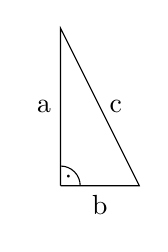
\begin{tikzpicture}[scale=.5]
        \begin{scope}[rotate=0] 
        \draw (0,0) -- node[below] {b} (2,0) -- node[right] {c} (0,4) -- node[left] {a} (0,0);
        \draw (0.5, 0) arc [start angle=0, end angle=90, radius=0.5];
        \draw (0.2,0.2) node {$\cdot$};
        \end{scope}
        \end{tikzpicture}
\end{minipage}%
\begin{minipage}{0.85 \textwidth}
\begin{parts}
    \part[1] Kreuze die richtige Formel für die Berechnung der \textbf{Hypotenusenlänge} an. \hier
    
    \begin{oneparcheckboxes}
        \choice $c=\sqrt{a+b}$
        \choice $c=a+b$%$
        \choice $c=\sqrt{a^2+b^2}$
        \choice $c=a^2+b^2$
    \end{oneparcheckboxes} \droppoints
    \part[1] Kreuze die richtige Formel für die Berechnung der \textbf{Kathetenlänge} an. \hier
    
        \begin{oneparcheckboxes}
        \choice $a=\sqrt{c+b}$
        \choice $a=\sqrt{c^2+b^2}$
        \choice $a=c-b$%$
        \choice $a=\sqrt{c^2-b^2}$
    \end{oneparcheckboxes} \droppoints
\end{parts}
\end{minipage}

\droptotalpoints
\newpage
\question[4]
Berechne die fehlenden Seitenlängen der unten abgebildeten Dreiecke. \medskip

    \begin{minipage}{0.5 \textwidth}
        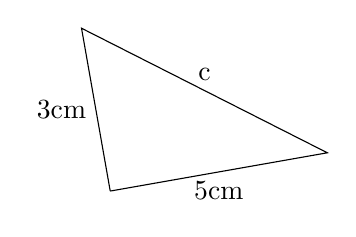
\begin{tikzpicture}[scale=.7]
        \begin{scope}[rotate=10] 
        \draw (0,0) -- node[below] {5cm} (4,0) -- node[above] {c} (0,3) -- node[left] {3cm} (0,0);
        %\draw (0.5, 0) arc [start angle=0, end angle=90, radius=0.5];
        %\draw (0.2,0.2) node {$\cdot$};
        \end{scope}
        \end{tikzpicture}
    \end{minipage}%
        \begin{minipage}{0.3 \textwidth}
        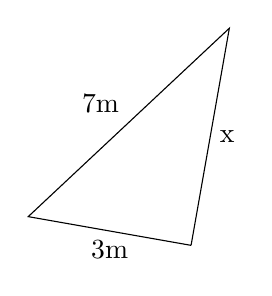
\begin{tikzpicture}[scale=.7]
        \begin{scope}[rotate=80] 
        \draw (0,0) -- node[right] {x} (4,0) -- node[above left] {7m} (0,3) -- node[below] {3m} (0,0);
        %\draw (0.5, 0) arc [start angle=0, end angle=90, radius=0.5];
        %\draw (0.2,0.2) node {$\cdot$};
        \end{scope}
        \end{tikzpicture}
    \end{minipage}
    
\droptotalpoints

\question[3]
Bring die folgenden Schritte in die Reihenfolge zur Anwendung des Satzes des Pythagoras. Setze dazu die Zahlen 1 bis 4 in die Lücken ein. \hier

\item[\loeslin \textbf{Schritt:}] Schreibe die richtige Formel auf.
\item[\loeslin \textbf{Schritt:}] Überlege, ob die Hypotenusenlänge oder die Kathetenlänge gesucht ist.
\item[\loeslin \textbf{Schritt:}] Benenne die Seiten und trage die bekannten Größen ein.
\item[\loeslin \textbf{Schritt:}] Markiere das rechtwinklige Dreieck und den rechten Winkel.


\droptotalpoints
\begin{comment}
\question[3]\
Ein Rechteck ist  30 cm breit und 17 cm breit. Berechne die Länge der Diagonale auf zwei Stellen genau. Fertige hierzu eine \underline{Skizze} an.

\medskip

\droptotalpoints
\end{comment}
\question[4]

\begin{minipage}{0.4 \textwidth}
    \includegraphics[scale=0.7]{bilder/spielfeld_american_football.png}
\end{minipage}%
\begin{minipage}{0.55 \textwidth}
    Beim American Football hat das Spielfeld die Maße 109,7m x 48,5m. Wie viel Meter legt ein Spieler zurück, der die Strecke diagonal läuft? 
    
    Fertige eine Skizze an und berechne die Strecke!
\end{minipage}

\droptotalpoints

\question[4]

\begin{minipage}{0.4 \textwidth}
  \includegraphics[scale=1]{bilder/pythagoras_drachen.PNG}
\end{minipage}%
\begin{minipage}{0.55 \textwidth}
  Robert und Sandra lassen einen Drachen steigen. Robert hält die vom
  Wind straff gespannte 80 m lange Drachenschnur. Sandra stellt sich
  genau unter den Drachen. Sie ist 60 m von Robert entfernt. Wie hoch
  steht der Drachen? 
\end{minipage}

\droptotalpoints

\newpage
\question[4]
\begin{minipage}{0.4\textwidth}
    \includegraphics[scale=0.25]{pythagoras_leiter.PNG}
\end{minipage}%
\begin{minipage}[b]{0.5\textwidth}
    Die abgebildete Leiter hat in zusammengeklapptem Zustand eine Länge von 2,50 Meter. Die Standbreite in ausgeklapptem Zustand beträgt 1,3 Meter. Wie hoch ist die Leiter?
\end{minipage}

\droptotalpoints
\question

\begin{minipage}{0.5 \textwidth}
\begin{center}
\pgfplotsset{
  compat=1.12,
  axis lines=middle
}
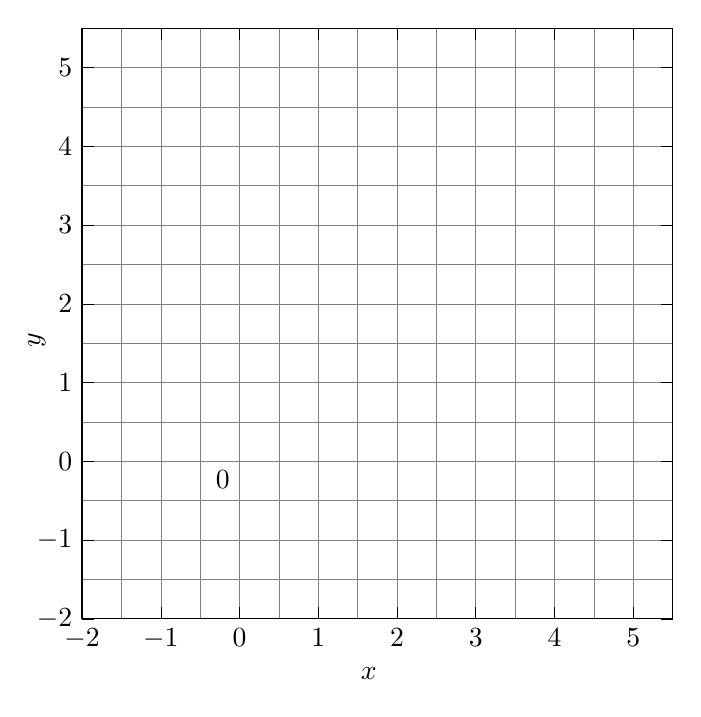
\begin{tikzpicture}
  \begin{axis}[
    xlabel=$x$,
    xlabel style={below, anchor=north east,inner xsep=0pt},
    ylabel=$y$,
    ylabel style={above,anchor=north east,inner ysep=0pt},
    xmin=-2,xmax=5.5,
    ymin=-2,ymax=5.5,
    x=1cm,
    y=1cm,
    tick style=black,
    restrict y to domain=-10:10,
    set layers
    ]
    \pgfplotsinvokeforeach {-10,-9.5,...,10}{
      \pgfonlayer{axis grid}
        \begin{scope}
          \clip(current axis.south west)rectangle(current axis.north east);
          \draw[help lines](#1,0|-current axis.south)--(#1,0|-current axis.north);
          \draw[help lines](0,#1-|current axis.west)--(0,#1-|current axis.east);
        \end{scope}
      \endpgfonlayer
    }
    \node [anchor=north east] at (0, 0) {$0$};
  \end{axis}
\end{tikzpicture}
\end{center}
\end{minipage}%
\begin{minipage}[b]{0.45 \textwidth}
    \begin{parts}
    \part[2] Trage die Punkte in das nebenstehende Koordinatensystem ein. \hier \droppoints \vspace*{-1cm}
    \begin{align*}
        &A(2|1)
        &B(5|5)
    \end{align*}
    \part[2]
Berechne den Abstand zwischen Punkt A und Punkt B. \droppoints
    \end{parts}
\end{minipage}

\droptotalpoints


\question
\begin{minipage}{0.3 \textwidth}
    \includegraphics[scale=0.7]{pythagoras_umkehrung.PNG}
\end{minipage}%
\begin{minipage}{0.65 \textwidth}
    Betrachte das unregelmäßige Viereck auf der linken Seite.
    \begin{parts}
    \part[3] Zeige durch Rechnung, dass der Winkel in Punkt B kein rechter Winkel ist. \droppoints
    \part[3] Bewerte, ob der Winkel im Punkt D annähernd ein rechter Winkel ist. \droppoints
    \end{parts}
\end{minipage}

\droptotalpoints

\begin{comment}

\question[6] Überprüfe durch Rechnung, welche der Dreiecke wirklich einen rechten Winkel besitzt.

\begin{minipage}{0.3\textwidth}
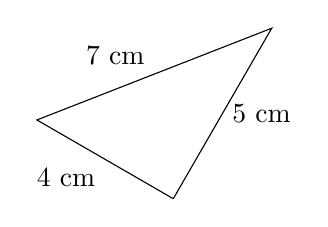
\begin{tikzpicture}[scale=0.5]
  \draw[rotate=-30,shift={(0 cm,0 cm)}] (0,0) -- node[below left]{$4$ cm}(-4,0) -- node[above left]{$7$ cm} (0,5) -- node[right]{$5$ cm}(0,0);
\end{tikzpicture}
\end{minipage}
\begin{minipage}{0.3\textwidth}
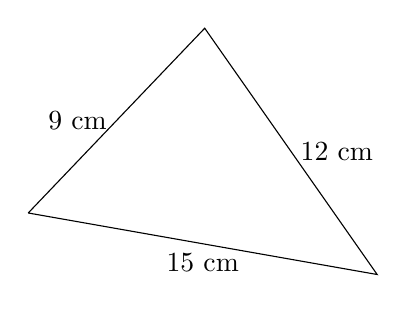
\begin{tikzpicture}[scale=0.3]
  \draw[rotate=-10,shift={(0 cm,0 cm)}] (-6,0) -- node[below]{$15$ cm}(9,0) -- node[right]{$12$ cm} (0,9) -- node[left]{$9$ cm}(-6,0);
\end{tikzpicture}
\end{minipage}
\begin{minipage}{0.3\textwidth}
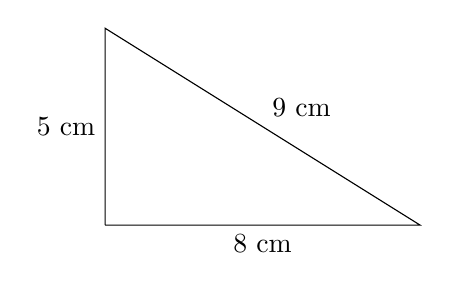
\begin{tikzpicture}[scale=0.5]
  \draw[rotate=0,shift={(0 cm,0 cm)}] (0,0) -- node[below]{$8$ cm}(8,0) -- node[above right]{$9$ cm} (0,5) -- node[left]{$5$ cm}(0,0);
\end{tikzpicture}
\end{minipage}\\[0.01cm]

\droptotalpoints
\end{comment}
\nomorequestions
\end{questions}
\end{document}